\documentclass[11pt,twocolumn]{article}
\usepackage{graphicx}
\usepackage[margin=1in]{geometry}
\usepackage{natbib}
\usepackage{amsmath, amssymb, graphicx}
\usepackage{authblk}
\usepackage{url}

\renewcommand\Authfont{\normalsize}
\renewcommand\Affilfont{\small}
\setlength{\affilsep}{0pt}

\providecommand{\apj}{ApJ}
\providecommand{\apjl}{ApJL}
\providecommand{\apjs}{ApJS}
\providecommand{\aap}{A\&A}
\providecommand{\mnras}{MNRAS}
\providecommand{\na}{New Astronomy}
\providecommand{\nat}{Nature}
\providecommand{\jaavso}{JAAVSO}
\providecommand{\aj}{AJ}
\providecommand{\araa}{ARA\&A}
\providecommand{\jcap}{JCAP}
\providecommand{\pasp}{PASP}

\begin{document}

\title{\textbf{Reproducing the Hubble Tension}}
\author{Brodie Monohan}
\affil{\textit{Whitman College}}

\date{May 10, 2026}

\twocolumn[
\begin{@twocolumnfalse}
\maketitle

\begin{abstract}
The Hubble Tension is one of the most pressing issues in modern cosmology. Independent measruements of the expansion rate of the universe using early and late universe phenomena disagree by around $5 \sigma$. Astronomers who extrapolate the expansion rate from the Cosmic Microwave Background (CMB) find a significantly lower value than the classical measurements of late universe objects like type 1a supernova. This tension indicates that the modern cosmological model is in some way incomplete. In this paper I recreate the Hubble Tension by measuring both early and late universe expansion rates using~\cite{Planck2018-Data} data of CMB anisotropies and~\cite{Pantheon2022_data} data of type 1a supernovae.
\end{abstract}

\vspace{1cm}
\end{@twocolumnfalse}
]

\section{Introduction}

The modern cosmological story starts with the Big Bang. Most people today have heard of the Big Bang, the event from which our universe and all its matter, energy, geometry, and foundational principles and mechanics began. The Big Bang was first theorized by Georges Lemaitre around 1930~\citep{ANHM} and has since been widely supported by observation. Some of the most notable are Leavitt and Hubble's discovery of galaxies and their recession~\citep{Hubble1929} and Penzias and Wilson's discovery of the Cosmic Microwave Background (CMB)~\citep{Penzias1965}. From these observations and many more in the last century, a robust theoretical history of the universe formed.

After the Big Bang, the universe rapidly began to expand and cool. In the first fractions of a second the universe passed through a sequence of distinct epochs, including inflation, the separation of fundamental forces, the formation of matter and antimatter, the formation of quarks and leptons, and finally the formation of electrons, protons, and neutrons. During this time the universe was extremely hot, near $\rm 10^{32}\ K$. Because of this, the energy density of the universe was also quite high, higher than the binding energy of the primordial elements, hydrogen and helium. This meant by the time of nucleosynthesis and the primordial elements had formed, they could not bind to electrons. By 1 second after the Big Bang, a primordial plasma dominated by photons, electrons, and the ionized primordial elements pervaded the universe. In this plasma, small quantum fluctuations created over-densities in some regions and under-densities in others. Over the next $\sim 380,000\rm yr$, these fluctuations grew into large scale oscillations. Much like the opacity mechanisms in variable stars\footnote{BAO acoustic waves are driven by radiation pressure and gravity, whereas $\kappa$ mechanisms involve opacity modulation of radiative diffusion but the overall mechanisms are similar}, these oscillations were driven via over-dense areas increasing in pressure as they contract gravitationally until the outward pressure overcomes the gravitational attraction and pushes the baryonic matter into the under-dense areas, turning them into the over-dense areas and starting the cycle over. These oscillations are called the Baryon Acoustic Oscillations (BAO). The waves that formed were on a broad spectrum of scales. 

During this time, the photons and free electrons interacted heavily through Thompson scattering which meant that the spatial distribution of baryons controlled the spatial distribution of photons as well. As expansion continued, the Universe eventually cooled enough for hydrogen and helium nuclei to combine with free electrons, transforming a once opaque universe into one where photons traveled freely. At this moment\footnote{Recombination (electrons binding with nuclei) and Decoupling (photons decoupling from electrons and baryonic matter) were not at the same ``moment'', nor did they happen all at once, creating features that CMB astronomers must consider} the Cosmic Microwave Background (CMB) was born, and in it, the distribution of matter which corresponded to the BAO waves was imprinted on it. Importantly, the largest fluctuations that were imprinted were those that were at maxima or minima in their oscillations at the moment of recombination. Modes that completed an integer fraction of a full oscillation by recombination were caught at an extrema and appear as the dominant patterns in the CMB, what we think of as the fundamental and harmonic modes.

\subsection{The CMB}
While investigating a persistent source of noise in the Holmdel Horn Antenna radio telescope,~\cite{Penzias1965} discovered the Cosmic Microwave Background. The CMB as we see it today originated $\sim \rm 380,000yr$ after the Big Bang when the universe had cooled enough for free electrons and protons to combine into $\sim 90\%$ neutral hydrogen and helium, and the once opaque universe allowed photons to travel freely with the BAO imprinted on them. Today, this remnant radiation of the Big Bang has been stretched with the expansion of the universe to the wavelength regime of microwaves. In 1989, NASA launched the Cosmic Background Explorer (COBE) which was aimed specifically at observing the CMB in high detail. With COBE data,~\cite{Smoot1992} discovered small temperature anisotropies in the CMB amounting to 1 part in $10^{6}$ which have since been attributed to the BAO\@. Because of this, these tiny temperature anisotropies encode information about the composition and geometry of the early universe that has had huge impacts on cosmology.

\subsection{The Modern Hubble Tension}
From the anisotropies in the CMB in combination with $\rm \Lambda CDM$ physical constraints, astronomers can measure the expansion rate of the universe ($H_0$). From the Planck Collaboration and a combination of Planck and Wilkinson Microwave Anisotropy Probe (WMAP) data,~\cite{Planck2018-Parameters} was able to measure $H_0$ by measuring the size and temperature of the anisotropies, particularly the anisotropies corresponding to the fundamental mode, and fitting this data to comprehensive $\Lambda \rm CDM$ models which are independently well supported. These measurements, however, yield a result that is in contention with classical $H_0$ measurements which rely on nearby late universe objects, most commonly supernovae. Multiple surveys from the past two decades have independently measured $H_0$ values that are in $\sim 5\sigma$ tension with values reported by teams measuring $H_0$ via the CMB\@. In this paper I produce early and late universe $H_0$ measurements and review the typical methodology.

\begin{figure}
    \centering
    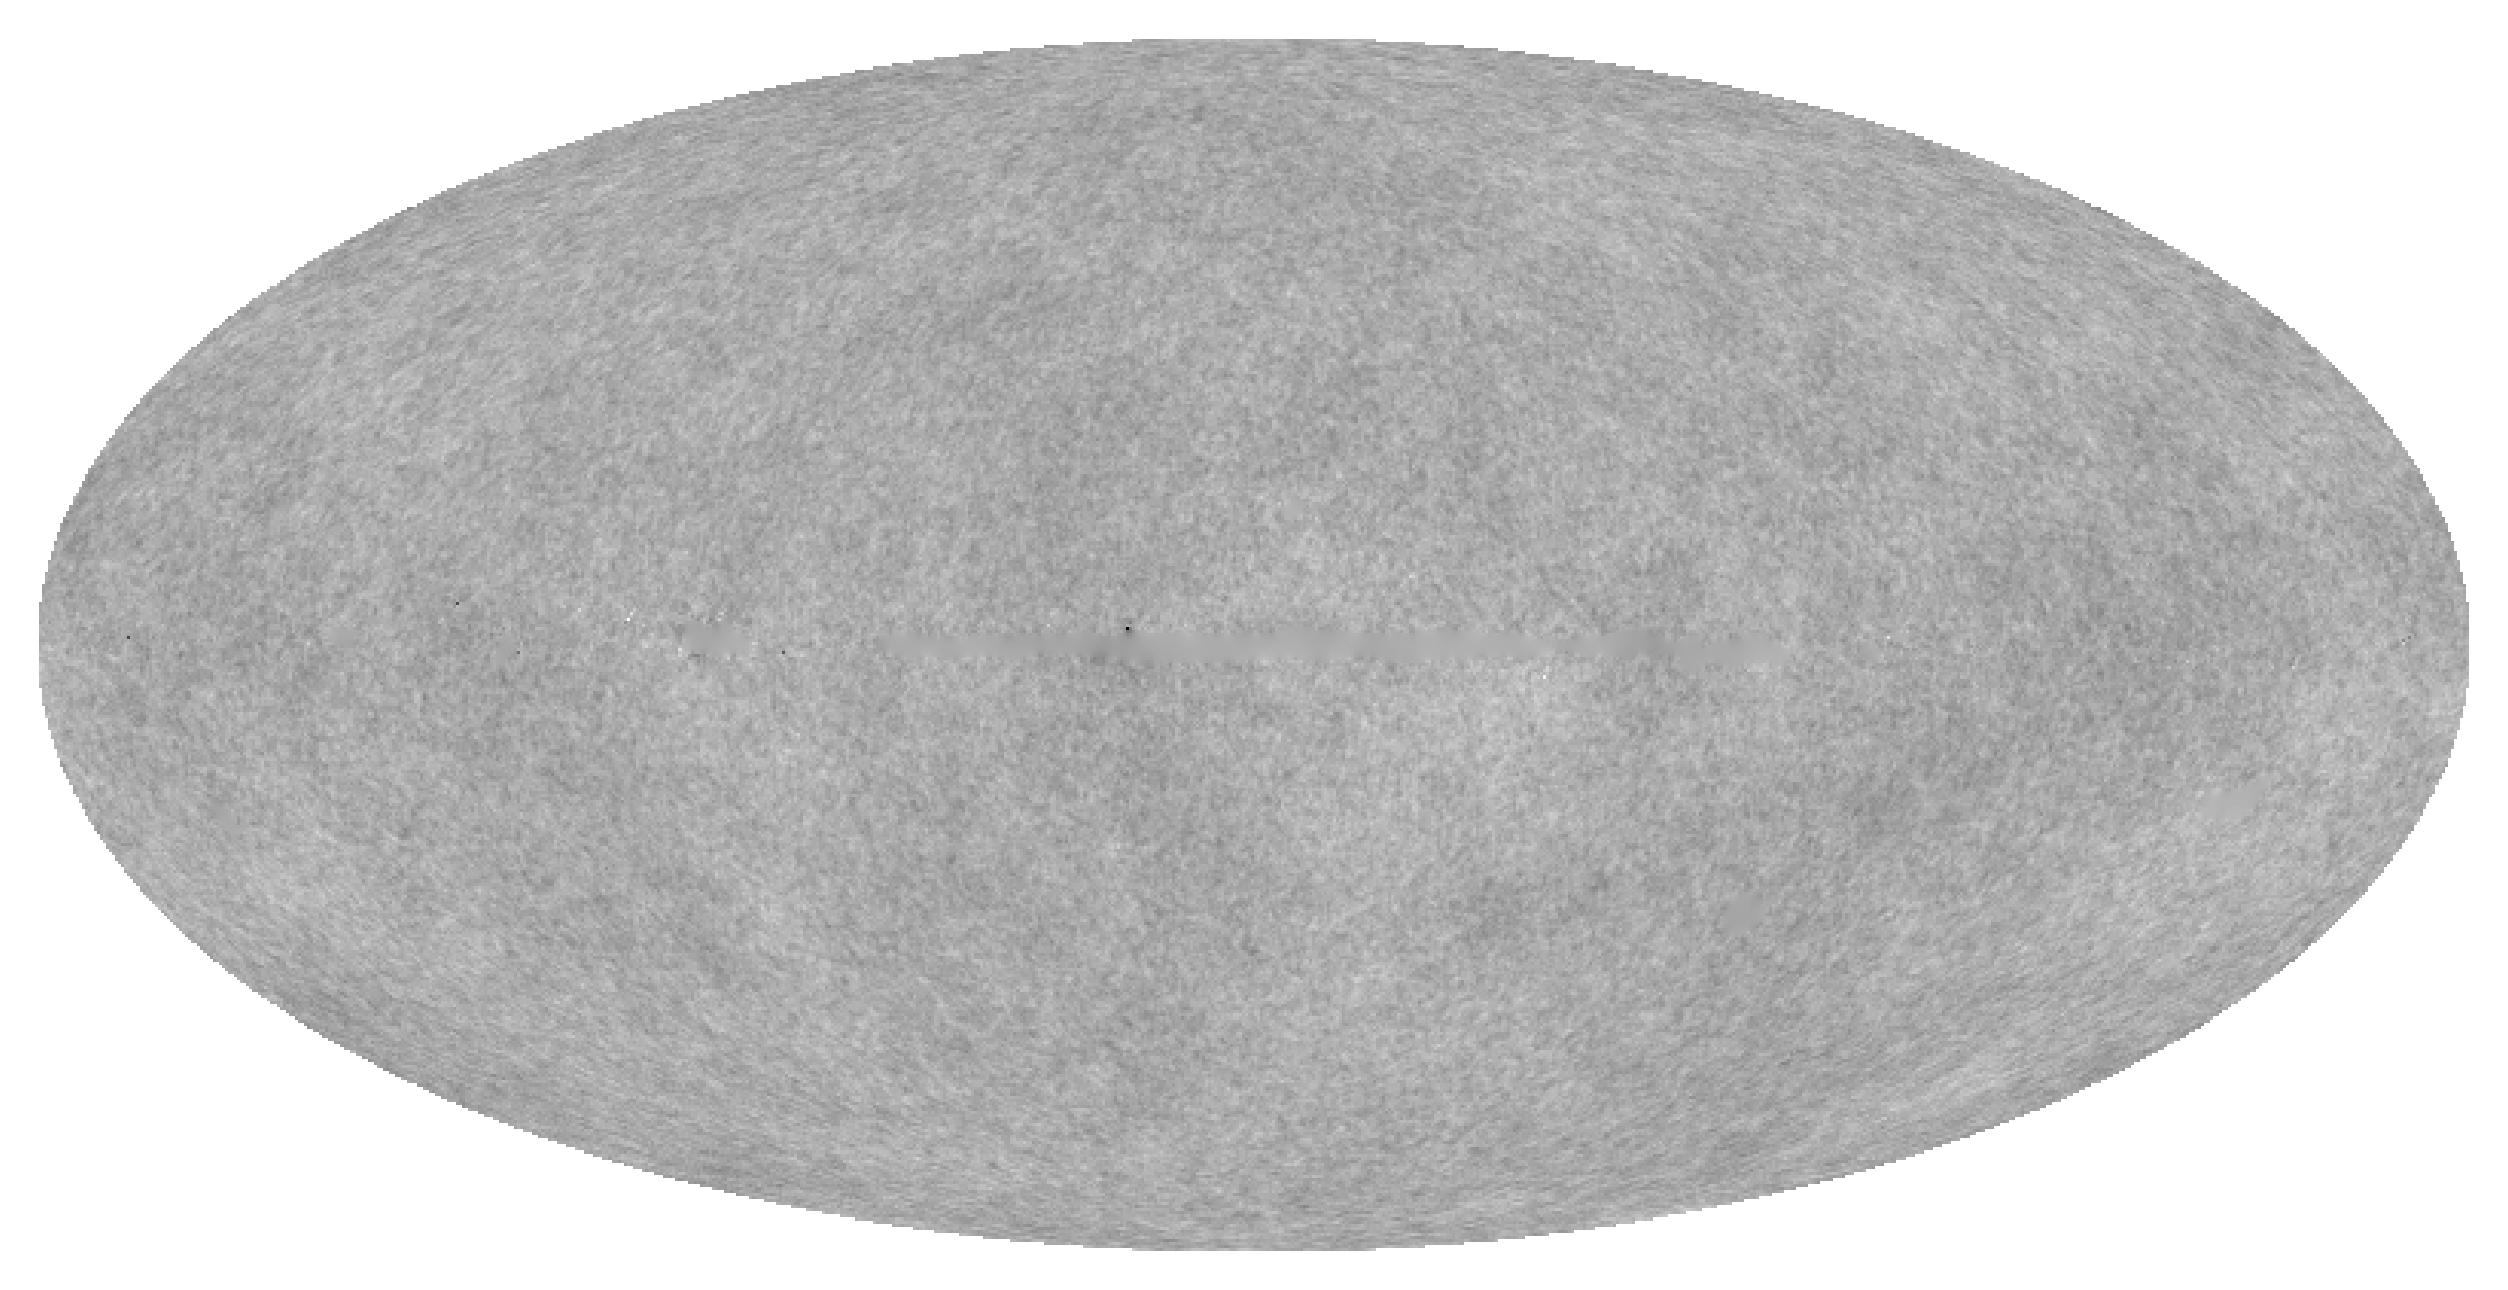
\includegraphics[width=0.49\textwidth]{../figures/cmb.jpeg}
    \caption{The processed Planck full mission data from~\cite{Planck2018-Data} as a Mollweide projection.}\label{fig:Planck_data}
\end{figure}

\begin{figure*}
    \centering
    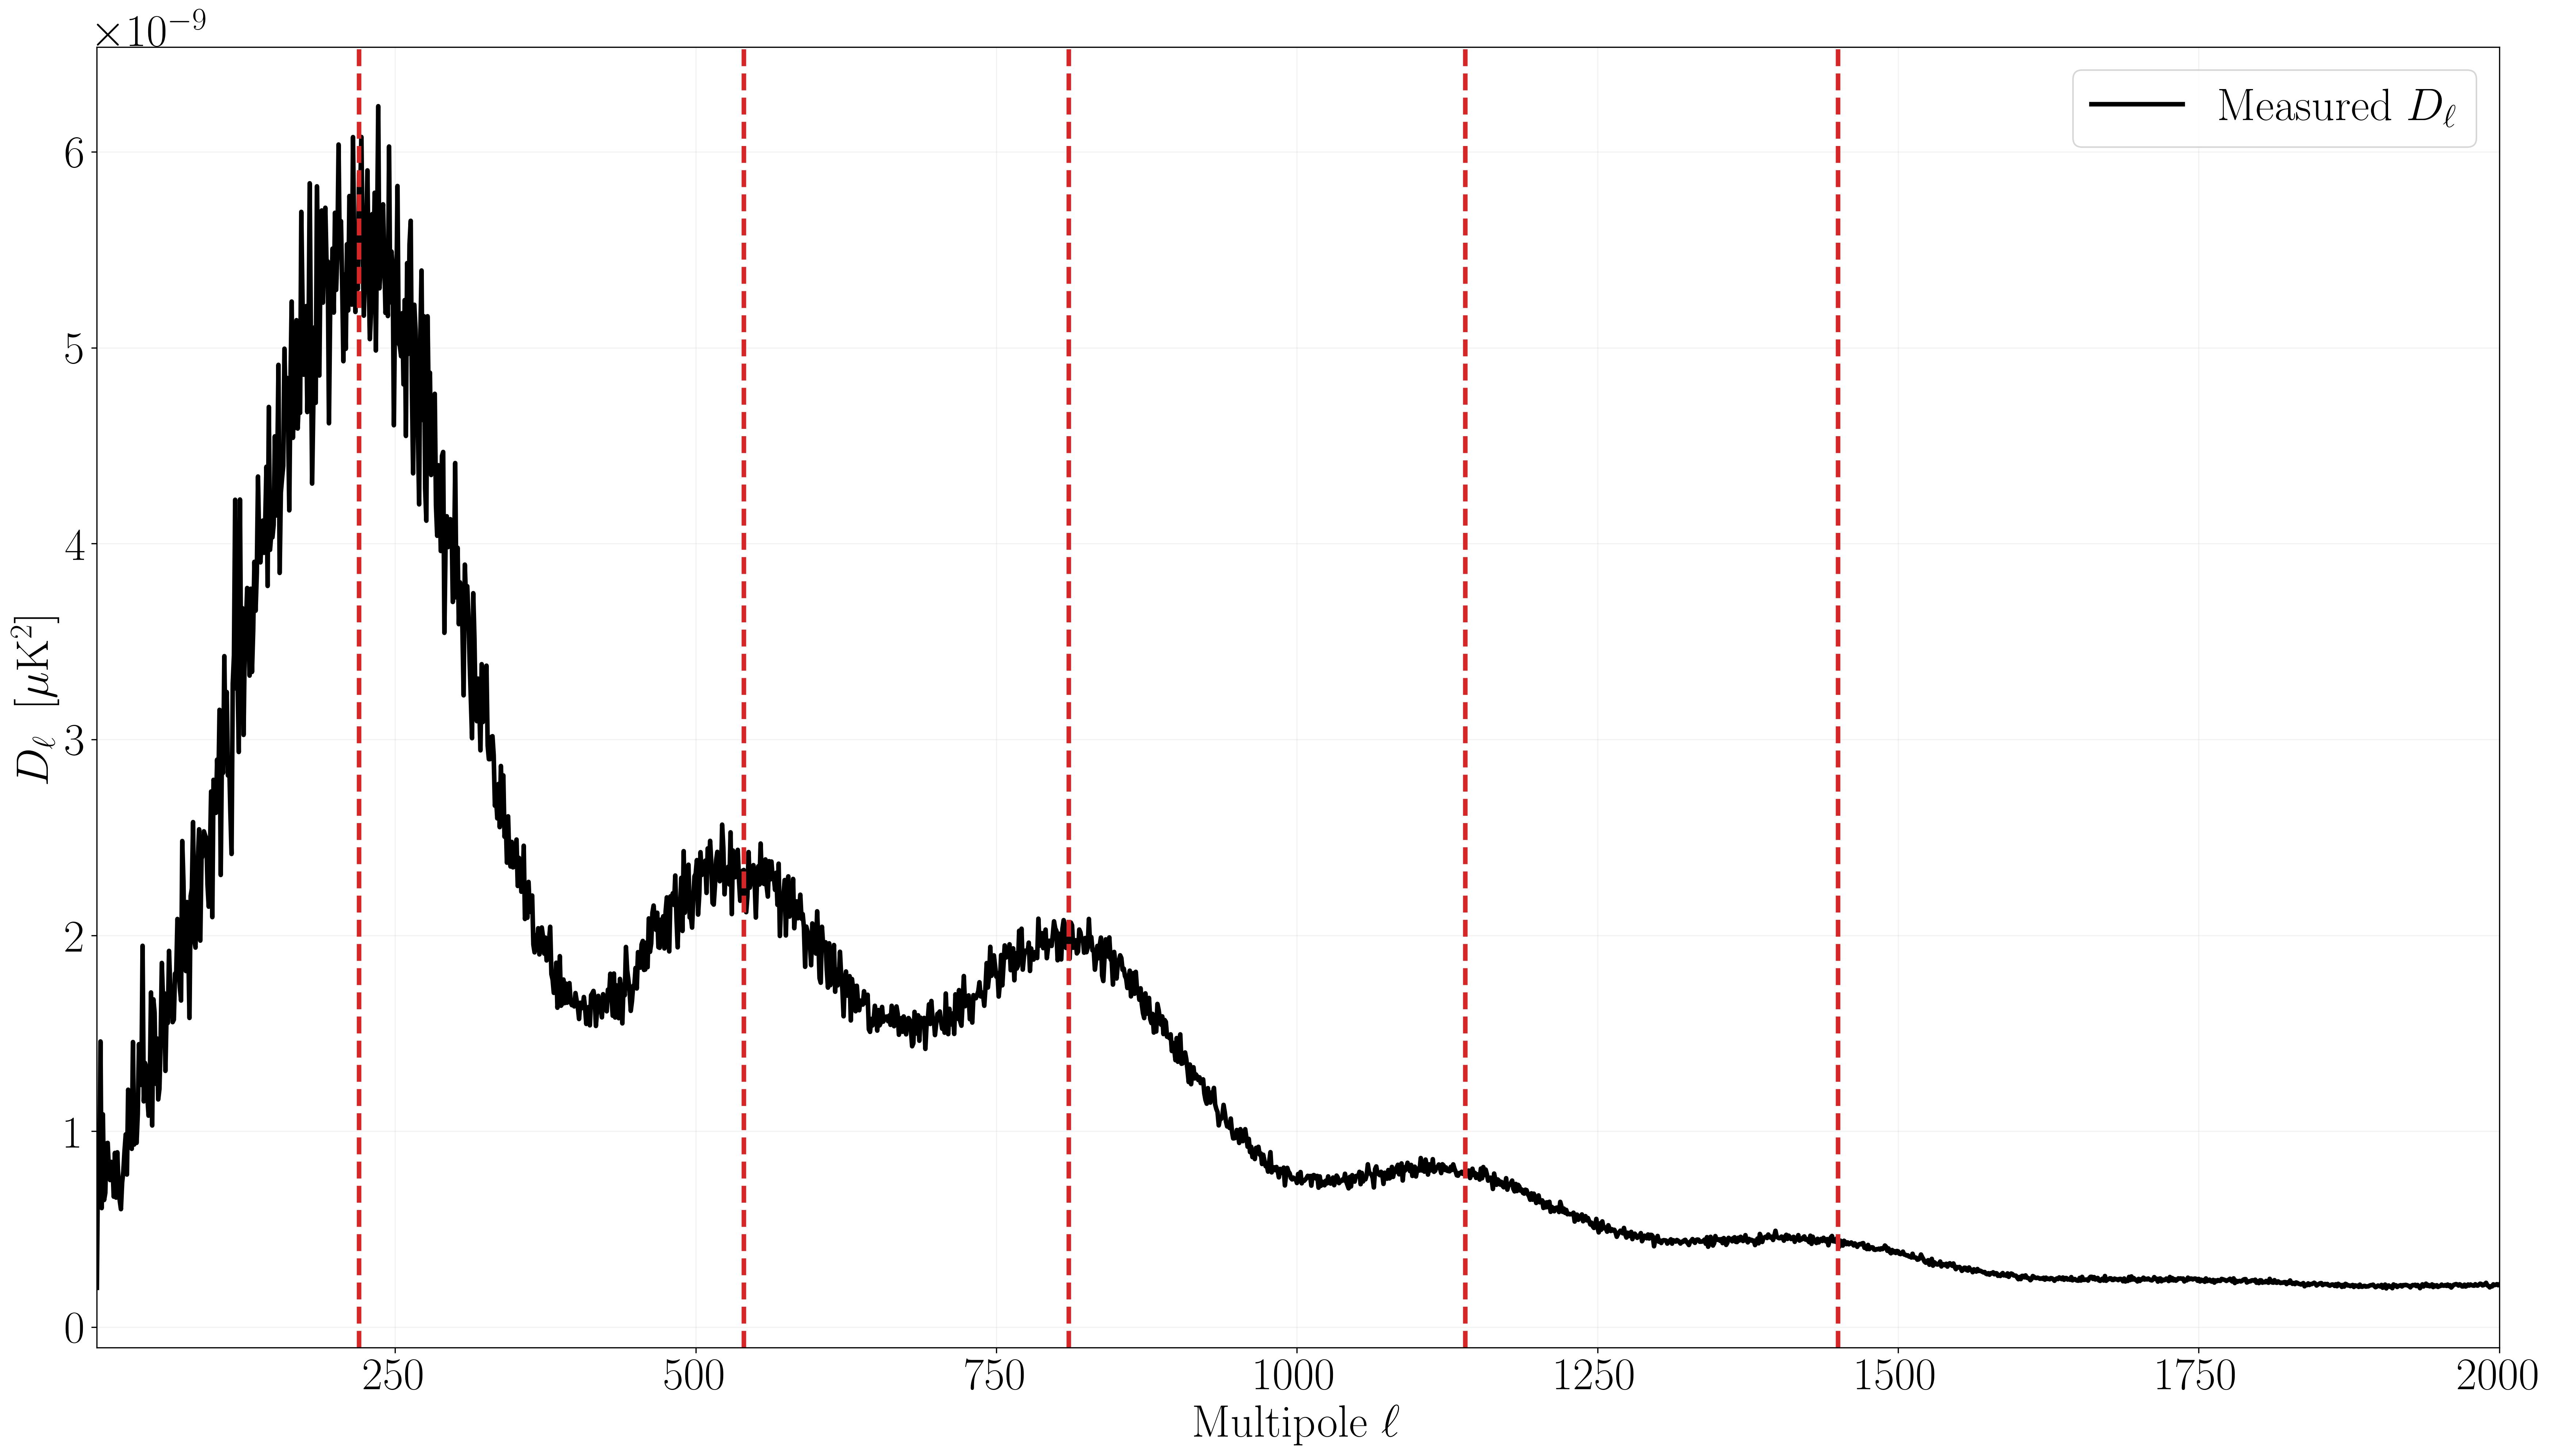
\includegraphics[width=\textwidth]{../figures/cmb_power_spectrum.jpeg}
    \caption{The $D_\ell$ power spectrum of the Plank full mission data from~\cite{Planck2018-Data} as a function of the multipole $\ell$ with the dominant multipoles as identified by~\cite{Planck2018-Parameters} plotted in red.}\label{fig:Power_spec}
\end{figure*}

\section{Data}
For an early universe calculation of $H_0$ I use Planck Legacy Archive full mission data from~\cite{Planck2018-Data} as seen in Figure~\ref{fig:Planck_data}. The early universe calculations rely on both a power spectrum fit and comprehensive $\Lambda \rm CDM$ model to constrain parameters. For the spectrum fit, I produce the power spectrum and compare to values obtained by~\cite{Planck2018-Parameters}. For the $\Lambda \rm CDM$ modeling, I rely completely on~\cite{Planck2018-Parameters}. For the late universe calculation of $H_0$ I use the Pantheon+SH0ES data from~\cite{Pantheon2022_data} and~\cite{SH0ES2022}, and super nova magnitude calibration from~\cite{SN_cal}.

\section{Analysis}

\subsection{Early Universe $H_0$}



Here I use the Planck Legacy Archive full mission data from~\cite{Planck2018-Data} to determine an angular size of the anisotropic patches $\theta$. To do this I can represent the CMB surface as a linear combination of spherical harmonic basis states. Spherical harmonics are the fundamental oscillating patterns on a sphere's surface much like sines and cosines form 2D harmonics for a circle. Importantly, the spherical harmonics $Y_{\ell m}$ form an orthonormal basis so any patterns on the surface of a sphere can be broken down into a linear combination of these basis states (much like a Fourier transform can break down a complex signal into a linear combination of sines and cosines). To find $\theta$ I can represent the Planck Legacy Archive data as an angular power spectrum 
\begin{equation}
    C_\ell = \langle| a_{\ell m}|^2\rangle
\end{equation}
which is the variance of the of the spherical harmonics whose coefficients are $a_{\ell m}$. $C_\ell$ is a function of $\ell$, the angular scale called the multipole defined as
\begin{equation}\label{ell}
    \ell \approx \pi/\theta
\end{equation}
The raw power spectrum, while it contains all of the information about the strength of signals at all frequencies, is not super useful on it's own and that is because of the geometry of spherical harmonics. At low $\ell$ oscillations (large angular size $\theta$ patterns), there are only a few ways these modes can be oriented producing only a few $a_{\ell m}$ coefficients. For large $\ell$ oscillations (small, fine angular size $\theta$ patterns) the number of $a_{\ell m}$ coefficients increases dramatically. For a scale-invariant power spectrum, $C\ell$ scales as $1/\ell(\ell+1)$ at low $\ell$. What we are interested in is not this geometrical artifact, but how $C_\ell$ deviates from it. Multiplying by $\ell(\ell+1)/2\pi$ produces a quantity that is approximately flat at low $\ell$, making deviations from scale-invariance and the acoustic peaks apparent. This gives $D_\ell$ which is the the contribution to total sky variance per logarithmic interval in $\ell$ which has units of $\mu K^2$~\citep{Planck2018-Parameters}. The $D_\ell$ power spectrum is shown in Figure~\ref{fig:Power_spec} as well as the monopoles corresponding to the dominant harmonics as identified by~\cite{Planck2018-Parameters}. From this spectrum they find an angular size of the first harmonic $\theta = 0.0104108 \pm 0.00031 \ \rm radians$ via equation~\ref{ell}. $\theta$ alone cannot directly inform an expansion history of the universe; to translate this into $H_0$, astronomers must determine a physical scale that these angles correspond to via
\begin{equation}
    \theta=\frac{r_s}{D_A}
\end{equation}
where $r_s$ is the physical size of the fluctuation and $D_A$ is the angular diameter distance to the surface of the CMB\@. If $r_s$ can be determined by physical constraints from $\rm \Lambda CDM$ (essentially what would we expect $r_s$ to be from running comprehensive $\rm \Lambda CDM$ models to produce the CMB spectrum we see today), then we can determine the distance to the CMB which will inform an expansion history of the universe. If we assume a flat universe, then 
\begin{equation}
    D_A =\frac{1}{1+z}\frac{c}{H_0}\int_0^z\frac{H(z)}{H_0}dz
\end{equation}
which isn't much useful on its own here (this is somthing that would be baked into a comprehensive $\rm \Lambda CDM$ model) but it illustrates the $H_0$ dependence well. By fitting the Planck spectrum using two programs (\texttt{Plik} and \texttt{CAMSpec})~\cite{Planck2018-Parameters} produces $\ell$ values for each dominant harmonic as well as fit cosmological parameters such as $\Omega_b$ (baryon density), $\Omega_c$ (cold dark matter density), and $A_s$ (the amplitude of primordial fluctuations). These models yield $H_0 \approx 67.3 \rm \ km \ s^{-1}\ Mpc^{-1}$.

\subsection{Late Universe $H_0$}

to find a late universe $H_0$, I can measure the apparent magnitude of nearby Type Ia supernovae (SNe Ia). Since SNe Ia have known intrinsic luminosities, they can act as standard candles which translated directly into distances via the distance modulus.
\begin{equation}
    m_b-M_b=5\log_{10}(d)-5 \rightarrow d=10^{\frac{m_b - M_b +5}{5}}
\end{equation}

\begin{figure}
    \centering
    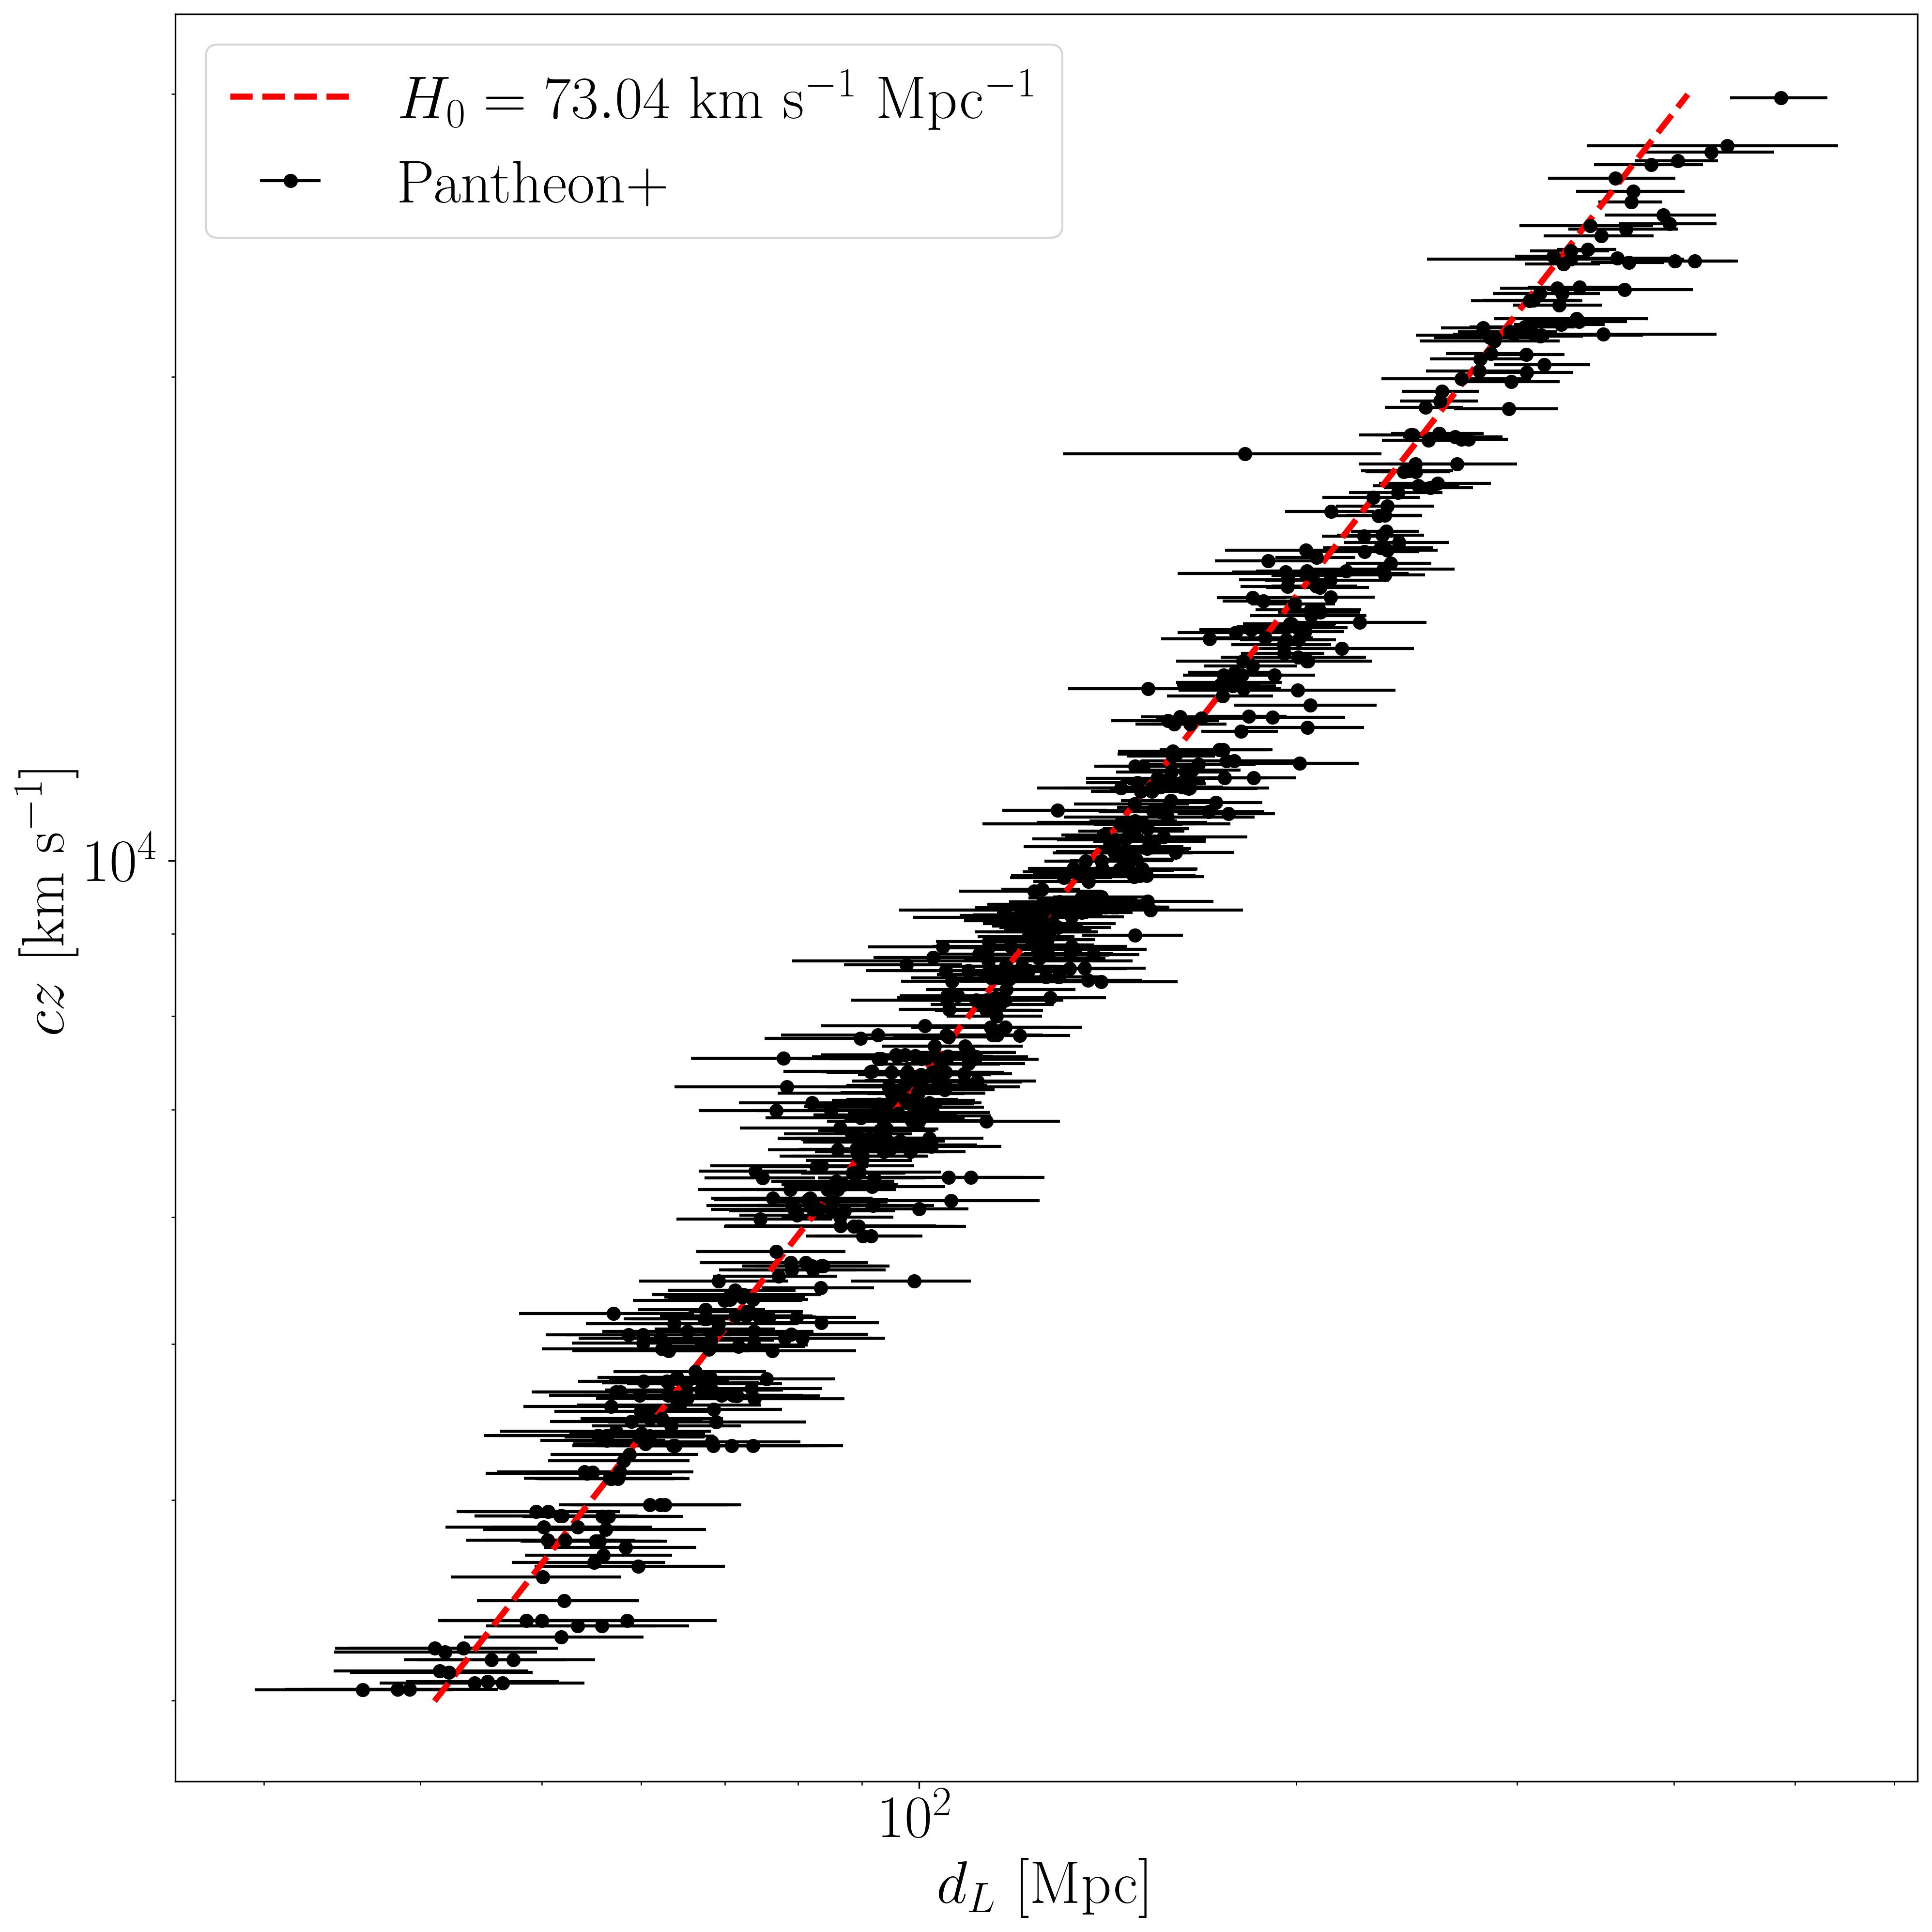
\includegraphics[width=0.5\textwidth]{../figures/SN_H_0.jpeg}
    \caption{The recession velocity of SNe 1a catalogued by~\cite{Pantheon2022_data} plotted as a function of distance with the linear best-fit $H_0$ identified by~\cite{Pantheon2022_parameters} plotted in red.}\label{fig:SNe_1a}
\end{figure}

To get a distance, I need to calibrate the absolute magnitude of supernovae which I can take from~\cite{SN_cal} as $M_B=-19.253\pm0.027$. I can then compare these distances ($d$) to the SNe Ia recession velocities ($v$) gained from redshift ($z$) to determine $H_0$ via
\begin{equation}
    v=H_0d \approx cz
\end{equation}

For nearby galaxies, $v\approx cz$. The Pantheon+/SH0ES sample measures spectroscopic redshift with corrections for local movement. With the Pantheon+/SH0ES sample I gather SNe Ia with redshifts $0.01<z<0.1$ and plot $cz$ vs $d$ with the $H_0 \approx 73 \rm \ km \ s^{-1}\ Mpc^{-1}$ measured by~\cite{Pantheon2022_parameters} fit over the data in Figure~\ref{fig:SNe_1a}.

\section{Discussion}

The Pantheon+/SH0ES value of $H_0 \approx 73 \rm \ km \ s^{-1}\ Mpc^{-1}$ sits in $5\sigma$ tension with the Planck CMB value of $H_0 \approx 67 \rm \ km \ s^{-1}\ Mpc^{-1}$, assuming a flat $\rm \Lambda CDM$ cosmology. This tension has been resilient to improvements in data/sensitivity which may signal a frontier of physics. Resolutions fall into a two broad categories. Early-universe solutions modify the pre-recombination physics. One of the most studied is the Early Dark Energy (EDE), a scalar field that contributes extra energy density before recombination which would raise $H_0$ as measured via the CMB~\cite{Doran2006}. Late-universe solutions modify the expansion history after recombination, suggesting a time dependent dark energy density. Currently, the Hubble tension remains one of the most pressing problems in cosmology, and the resolution is likely to have profound implications for the standard cosmological model.

\bibliographystyle{apalike}
\bibliography{ref}

\end{document}